\newpage
\section{ALU}

This module is a behavioral model of an Arithmetic Logic Unit (ALU) for a RISC-V  processor implemented in SystemVerilog. This ALU performs various arithmetic and logic operations based on the provided control signals. The module takes two 64-bit input operands and produces a 64-bit result. It also generates a zero flag to indicate whether the result is zero.

\subsection{Ports}

\begin{itemize}
    \item data01 (input, 64 bits): The first operand for the ALU operation.
    \item data02 (input, 64 bits): The second operand for the ALU operation.
    \item aluCtl (input, 4 bits): The control signal to specify the type of operation to be performed.
    \item aluOp (input, 2 bits): The high-level operation type signal, used for decoding the instruction class.
    \item zeroFlag (output, 1 bit): A flag that indicates whether the result is zero.
    \item result (output, 64 bits): The result of the ALU operation.
\end{itemize}



\begin{figure}[H]
    \centering
    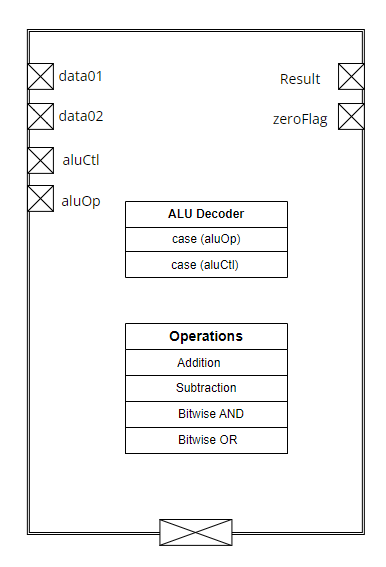
\includegraphics[width=0.4\linewidth]{Image/Block Diagram.png}
    \caption{ALU block diagram}
    \label{fig:ALU block diagram}
\end{figure}

\subsection{Parameters}
\begin{itemize}
    \item \textbf{loadOrStoreOp (2 bits):} Specifies load or store operation (2'b00).
    \item \textbf{branchOp (2 bits):} Specifies branch operation (2'bx1).
    \item \textbf{rTypeOp (2 bits)}: Specifies R-type operation (2'b1x).
    \item \textbf{store (4 bits): }Specifies store operation (4'b0010).
    \item \textbf{load (4 bits):} Specifies load operation (4'b0010).
    \item \textbf{branchIfEqual (4 bits):} Specifies branch if equal operation (4'b0110).
    \item \textbf{ariAdd (4 bits):} Specifies addition operation (4'b0010).
    \item \textbf{ariSub (4 bits):} Specifies subtraction operation (4'b0110).
    \item \textbf{bitAnd (4 bits):} Specifies bitwise AND operation (4'b0000).
    \item \textbf{bitOr (4 bits):} Specifies bitwise OR operation (4'b0001).
\end{itemize}

\subsection{ ALU Operation}
The ALU operation is decoded based on the aluOp and aluCtl signals. The following table summarizes the operations.



\begin{figure}[H]
    \centering
    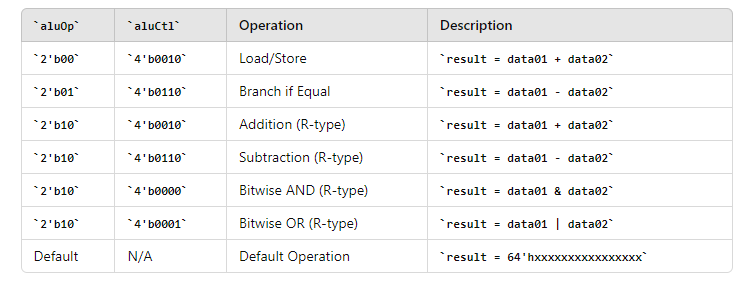
\includegraphics[width=0.5\linewidth]{Image/Alu truth table.png}
    \caption{ALU operation truth table}
    \label{fig:ALU operation truth table}
\end{figure}


\subsection{Detailed Functionality}
\begin{enumerate}
    \item Load/Store Operation (aluOp = 2'b00)
     \begin{itemize}
    \item Performs addition of data01 and data02.
     \item Sets zeroFlag if the result is zero.
     \end{itemize}
    
    \item Branch Operation (aluOp = 2'bx1)
    \begin{itemize}
     \item Performs subtraction of data01 and data02.
     \item Sets zeroFlag if the result is zero, indicating equality.
     \end{itemize}
     
    \item R-type Operation (aluOp = 2'b1x)
           \begin{itemize}
     \item Addition (aluCtl = 4'b0010): Adds data01 and data02.
    \item Subtraction (aluCtl = 4'b0110): Subtracts data02 from data01.
    \item Bitwise AND (aluCtl = 4'b0000): Performs bitwise AND between data01 and data02.
     \item Bitwise OR (aluCtl = 4'b0001): Performs bitwise OR between data01 and data02.
     \item Sets zeroFlag if the result of any operation is zero.
     \end{itemize}
    
    \item Default Operation
      \begin{itemize}
     \item Sets result to 64'hxxxxxxxxxxxxxxxx.
     \item Sets zeroFlag to 0.
     \end{itemize}
\end{enumerate}